
\section*{Problema P8.62}

\renewcommand*\thesection{8.62}
\numberwithin{equation}{section}

\begin{center}
    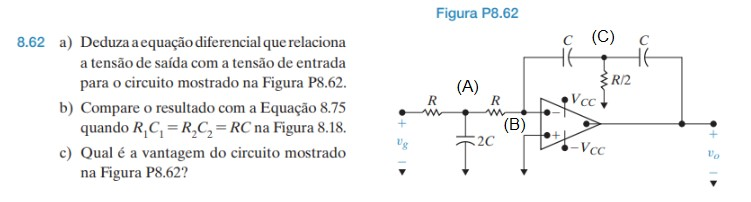
\includegraphics[scale=1.0]{P8.62.jpg}
\end{center}

\subsection*{(a)}

Usando o amplificador operacional como ideal, temos duas premissas que podemo tomar antes de começar a análise:

\begin{equation}\label{eq:8.62.1}
    V_+ = V_- = 0
\end{equation}

\begin{equation}\label{eq:8.62.2}
    i_+ = i_- = 0
\end{equation}

\eqref{eq:8.62.1} se refere ao curto circuito virtual entre os terminais de entrada do AmpOp, e \eqref{eq:8.62.2} se refere à impedância de entrada infinita;
Assim, temos três nós essenciais no circuito, nomeados (A), (B) e (C). Vamos aplicar análise nodal em cada um deles. \\
Nó (A): 

\[ \frac{V_A - v_g}{R} + i_C + \frac{V_A - 0}{R} = 0 \]

\[ \frac{V_A - v_g}{R} + 2C\diff{V_A}{t} + \frac{V_A}{R} = 0 \]

\[ \diff{V_A}{t} + \frac{V_A}{2RC} - \frac{v_g}{2RC} + \frac{V_A}{2RC} = 0 \]

\begin{equation}\label{eq:8.62.3}
    \diff{V_A}{t} + \frac{V_A}{RC} - \frac{v_g}{2RC} = 0
\end{equation}

Nó (B): 

\[ \frac{V_B - V_A}{R} + 0 + i_C = 0 \]

\[ \frac{V_B - V_A}{R} + C\diff{(V_B - V_C)}{t} = 0 \]

\[ \frac{V_B}{R} - \frac{V_A}{R} + C\diff{V_B}{t} - C\diff{V_C}{t} = 0 \]

Note que $V_B = 0$ devido à \eqref{eq:8.62.1}. Assim, 

\begin{equation}\label{eq:8.62.4}
    \frac{V_A}{R} + C\diff{V_C}{t} = 0
\end{equation}

Nó (C): 

\[ i_C + i_C + \frac{V_C}{0.5R} = 0 \]

\[ C\diff{(V_C - V_B)}{t} + C\diff{V_C - v_o}{t} + \frac{V_C}{0.5R} = 0 \]

\[ C\diff{V_C}{t} + C\diff{V_C}{t} - C\diff{v_o}{t} + \frac{V_C}{0.5R} = 0 \]

\begin{equation}\label{eq:8.62.5}
    2C\diff{V_C}{t} - C\diff{v_o}{t} + \frac{V_C}{0.5R} = 0
\end{equation}

A partir de \eqref{eq:8.62.4} é possível extrair duas informações: 

\[ V_A = - RC\diff{V_C}{t} \quad , \quad \diff{V_A}{t} = - RC\diff[2]{V_C}{t}  \]

Substituindo essas duas novas informações em \eqref{eq:8.62.3}, temos  

\[ - RC\diff[2]{V_C}{t} + \frac{- RC\diff{V_C}{t}}{RC} - \frac{v_g}{2RC} = 0 \]

\begin{equation}\label{eq:8.62.6}
    \diff[2]{V_C}{t} + \frac{1}{RC} \diff{V_C}{t} = - \frac{v_g}{2R^2C^2}
\end{equation}

Note que, diferenciando \eqref{eq:8.62.5}, temos  

\[ 2C\diff[2]{V_C}{t} - C\diff[2]{v_o}{t} + \frac{1}{0.5R} \diff{V_C}{t} = 0 \]

\begin{equation}\label{eq:8.62.7}
    \diff[2]{V_C}{t} + \frac{1}{RC} \diff{V_C}{t} = \frac{1}{2}\diff[2]{v_o}{t}
\end{equation}

Igualando os termos direitos das equações \eqref{eq:8.62.6} e \eqref{eq:8.62.7}, obtemos finalmente uma expressão da saída  
$v_o$ em função da entrada $v_g$.

\[  - \frac{v_g}{2R^2C^2} = \frac{1}{2}\diff[2]{v_o}{t} \]

\[ \boxed{\diff[2]{v_o}{t} = - \frac{v_g}{R^2C^2} } \]

\subsection*{(b)}

Se $R_1C_1$ = $R_2C_2$, temos  

\[ R_1C_1 \cdot R_2C_2 = R^2C^2 \]

E a equação 8.75 do livro se torna a mesma equação deduzida no item (a) do problema. A única diferença é que o circuito 
do problema inverte o sinal da entrada. 

\subsection*{(c)}

O circuito da Figura P8.62 é capaz ter a mesma função resposta do circuito da Figura 8.18 do livro usando apenas um 
amplificador operacional, ao passo que o do livro usa dois AmpOps. A única desvantagem é que ele também inverte o sinal, o que
pode ser indesejado em algumas aplicações.
